% !TeX root = mos-he.tex

%%%%%%%%%%%%%%%%%%%%%%%%%%%%%%%%%%%%%%%%%%%%%%%%%%%%%%%%%%%%%%%%

\begin{prob}{לדגום עם או בלי החזרות?}{D}{(Should you sample with or without replacement?)}

בכד 
$A$
נמצאים
$2$
כדורים אדומים וכדור ירוק אחד, ובכד 
$B$
נמצאים
$101$
כדורים אדומים ו-%
$100$
כדורים ירוקים. בחר כד אחד בצורה אקראי ושלוף שני כדורים באופן אקראי מהכד שנבחר. אתה מנצח אם אתה מזהה נכון אם כדורים נשלפו מכד 
$A$
או כד
$B$.

חשב את ההסתברויות לניצחון בכל אחד מהחוקים שלהן וקבע איזו שיטה נותן את ההסתברות הגבוהה ביותר לניצחון.

\que{1}
אתה מחזיר את הכדור הראשון לפני השליפה השנייה.

\que{2} 
אתה לא מחזיר את הכדור הראשון לפני השליפה השנייה.

\que{3}
לאחר שליפת הכדור הראשון אתה יכול להחליט אם להחזיר אותו או לא.

\textbf{רמז:} 
כאשר מחשבים הסתברויות:
\[
\disfrac{101}{201}\approx \disfrac{100}{201} \approx \disfrac{100}{200} \approx \disfrac{1}{2}\,.
\]
\end{prob}
\vspace{-6ex}

\solution{}

יש ארבע תוצאות שנסמן
$RR, RG, GR, GG$.
לכל אחד מהחוקים נחשב את ההסתברויות המתנות של ארבעת התוצאות כתלות בזהות הכד 
$A$
או
$B$
שנבחר תחילה. אחר כך נכפיל את ההסתברויות ב-%
$1/2$
כדי לקחת בחשבון את הבחירה האקראית של הכד.

\ans{1}
שליפה עם החזרה:
\[
\renewcommand*{\arraystretch}{1.5}
\begin{array}{lcccc}
P(RR|A) &=& \frac{2}{3} \cdot \frac{2}{3} &=& \frac{4}{9}\\
P(RR|B) &=& \frac{1}{2} \cdot \frac{1}{2} &=& \frac{1}{4}\\
\hline
P(RG|A) &=& \frac{2}{3} \cdot \frac{1}{3} &=& \frac{2}{9}\\
P(RG|B) &=& \frac{1}{2} \cdot \frac{1}{2} &=& \frac{1}{4}\\
\hline
P(GR|A) &=& \frac{1}{3} \cdot \frac{2}{3} &=& \frac{2}{9}\\
P(GR|B) &=& \frac{1}{2} \cdot \frac{1}{2} &=& \frac{1}{4}\\
\hline
P(GG|A) &=& \frac{1}{3} \cdot \frac{1}{3} &=& \frac{1}{9}\\
P(GG|B) &=& \frac{1}{2} \cdot \frac{1}{2} &=& \frac{1}{4}\end{array}
\]
אם התוצאה היא
$RR$
ההסתברות שכד 
$A$
נבחר
($4/9$)
גבוהה מהסתברות שכד
$B$
נבחר
($1/4$);
אחרת, ההסתברות ש-%
$B$
נבחר גבוהה יותר. לכן:
\[
P(\textrm{ניצחון})=\frac{1}{2}\left(\frac{4}{9} + \frac{1}{4}+ \frac{1}{4}+ \frac{1}{4}\right)=\disfrac{43}{72}\approx 0.5972\,.
\]

\ans{2}
שליפה ללא החזרה:
\[
\renewcommand*{\arraystretch}{1.5}
\begin{array}{lcccc}
P(RR|A) &=& \frac{2}{3} \cdot \frac{1}{2} &=& \frac{1}{3}\\
P(RR|B) &=& \frac{1}{2} \cdot \frac{1}{2} &=& \frac{1}{4}\\
\hline
P(RG|A) &=& \frac{2}{3} \cdot \frac{1}{2} &=& \frac{1}{3}\\
P(RG|B) &=& \frac{1}{2} \cdot \frac{1}{2} &=& \frac{1}{4}\\
\hline
P(GR|A) &=& \frac{1}{3} \cdot 1 &=& \frac{1}{3}\\
P(GR|B) &=& \frac{1}{2} \cdot \frac{1}{2} &=& \frac{1}{4}\\
\hline
P(GG|A) &=& \frac{1}{3} \cdot 0 &=& 0\\
P(GG|B) &=& \frac{1}{2} \cdot \frac{1}{2} &=& \frac{1}{4}
\end{array}
\]
אם התוצאה היא
$GG$
ההסתברות שכד
$B$
נבחר גבוהה יותר (כמובן!) מההסתברות שכד
$A$
נבחר; אחרת, ההסתברות שכד 
$A$
נבחר גבוהה יותר. לכן:
\[
P(\textrm{ניצחון})=\frac{1}{2}\left(\frac{1}{3} + \frac{1}{3}+ \frac{1}{3}+ \frac{1}{4}\right)=\frac{5}{8}=0.6250\,,
\]
שהיא גבוהה יותר מההסתברות לניצחון כאשר שליפה היא עם החזרה.

\ans{3} 
ההחלטה נעשית על סמך התוצאות של השליפה הראשונה.

אם השליפה הראשונה היא מכד
$A$
ההסתברויות חייבות להיות מותנות גם בהחלטה להחזיר או לא. אם השליפה הראשונה היא מכד
$B$
היא לא משפיעה על ההסתברויות בגלל הקירוב ברמז.
\[
\renewcommand*{\arraystretch}{1.5}
\begin{array}{lcccc}
P(RR|A,w) &=& \frac{2}{3} \cdot \frac{2}{3} &=& \frac{4}{9}\\
P(RR|A,w/o) &=& \frac{2}{3} \cdot \frac{1}{2} &=& \frac{1}{3}\\
P(RR|B) &=& \frac{1}{2} \cdot \frac{1}{2} &=& \frac{1}{4}\\
\hline
P(RG|A,w) &=& \frac{2}{3} \cdot \frac{1}{3} &=& \frac{2}{9}\\
P(RG|A,w/o) &=& \frac{2}{3} \cdot \frac{1}{2} &=& \frac{1}{3}\\
P(RG|B) &=& \frac{1}{2} \cdot \frac{1}{2} &=& \frac{1}{4}\\
\hline
%\end{array}
%\]
%\[
%\renewcommand*{\arraystretch}{1.5}
%\begin{array}{lcccc}
P(GR|A,w) &=& \frac{1}{3} \cdot \frac{2}{3} &=& \frac{2}{9}\\
P(GR|A,w/o) &=& \frac{1}{3} \cdot 1 &=& \frac{1}{3}\\
P(GR|B) &=& \frac{1}{2} \cdot \frac{1}{2} &=& \frac{1}{4}\\
\hline
P(GG|A,w) &=& \frac{1}{3} \cdot \frac{1}{3} &=& \frac{1}{9}\\
P(GG|A,w/o) &=& \frac{1}{3} \cdot 0 &=&0\\
P(GG|B) &=& \frac{1}{2} \cdot \frac{1}{2} &=& \frac{1}{4}\\\end{array}
\]
אם כדור אדום נשלף ראשונה אזי 
$\frac{4}{9}>\frac{1}{4}$
ו-%
$\frac{2}{9}<\frac{1}{4}$
עם החזרה, לעומת
$\frac{1}{3}>\frac{1}{4}$
ו-%
$\frac{1}{3}>\frac{1}{4}$
ללא החזרה, לכן הכדור השני יכול לעזור בזיהוי הכד רק אם השליפה נעשית 
\textbf{עם}
החזרה: אם אדום כד
$A$
ואם ירוק כד
$B$.
נבחר שליפה עם החזרה:
\[
P(\textrm{ראשון אדום אם ניצחון})=\frac{1}{2}\left(\frac{4}{9}+\frac{1}{4}\right)=\frac{25}{72}\,.
\]
אם כדור ירוק נשלף ראשון אזי
$\frac{2}{9}<\frac{1}{4}$
ו-%
$\frac{1}{9}<\frac{1}{4}$
עם החזרה, לעומת
$\frac{1}{3}>\frac{1}{4}$
ו-%
$0<\frac{1}{4}$
ללא החזרה, לכן הכדור השני יכול לעזור בזיהוי הכד רק אם השליפה נעשית 
\textbf{בלי}
החזרה:
\[
P(\textrm{ראשון ירוק אם ניצחון})=\frac{1}{2}\left(\frac{1}{3}+\frac{1}{4}\right)=\frac{7}{24}\,.
\]
ההסתברות לניצחון היא:
\[
P(\textrm{ניצחון})=\frac{25}{72} + \frac{7}{24}=\frac{23}{36}\approx 0.6389\,.
\]
ההסתברות הגבוהה ביותר לניצחון מתקבלת כאשר ההחלטה לשלוף עם או בלי החזרה מתקבלת בהתאם לתוצאה של השליפה הראשונה.

\textbf{סימולציה}
\selectlanguage{english}
\begin{verbatim}
With replacement:
Expectation of winning = 0.5972
Average wins           = 0.5976
Without replacement:
Expectation of winning = 0.6250
Average wins           = 0.6207
Decide after first draw:
Expectation of winning = 0.6389
Average wins           = 0.6379
\end{verbatim}
\selectlanguage{hebrew}

%%%%%%%%%%%%%%%%%%%%%%%%%%%%%%%%%%%%%%%%%%%%%%%%%%%%%%%%%%%%%


\begin{prob}{הקלפי}{}{(The ballot box)}

שני מועמדים
$A$
ו-%
$B$
מתמודדים בבחירות. 
$A$
קיבל
$a$
קולות ו-%
$B$
קיבל
$b$
קולות,
$a>b$.
הקולות נספרים אחד-אחד וסכומי הביניים
$(a_i,b_i), 1\leq i \leq a+b$
מתעדכנים לאחר ספירת כל קול. מה ההסתברות שעבור לפחות
$i$
אחד,
$a_i=b_i$?

\que{1} 
פתור עבור
$a=3, b=2$
על ידי הכנת רשימה
$(a_i,b_i)$
עבור
$1\leq i\leq 5$.

\que{2} 
פתור לכל
$a>b$.

\textbf{רמז 1:} 
מה ניתן להגיד על זהות המועמד המוביל עד לתיקו 
\textbf{הראשון}?

\textbf{Hint 2:}
מה החשיבות של הקול הראשון שנספר.
\end{prob}

\newpage

\solution{}

\ans{1}
מספר הדרכים לסדר את סכומי הביניים הוא
${5\choose 2}={5\choose 3}=10$ 
כי המיקום הקולות עבור מועמד אחד קובע את מיקום הקולות של המועמד השני. בטבלה שלהלן רשומים הסידורים האפשריים של הקולות וסכומי הביניים כאשר התיקו הראשון מודגש:
\begin{center}
\begin{minipage}{.48\textwidth}
\[
\begin{array}{ccccc}
A & A & A & B & B\\
A & A & B & A & B\\
A & B & A & A & B\\
B & A & A & A & B\\%\hline
A & A & B & B & A\\
A & B & A & B & A\\
B & A & A & B & A\\%\hline
A & B & B & A & A\\
B & A & B & A & A\\%\hline
B & B & A & A & A
\end{array}
\]
\end{minipage}
\hspace{-4em}
\begin{minipage}{.48\textwidth}
\[
\begin{array}{rrrrr}
%(4,5)&
(1,0) & (2,0) & (3,0) & (3,1) & (3,2)\\
%(3,5)&
(1,0) & (2,0) & (2,1) & (3,1) & (3,2)\\
%(2,5)&
(1,0) & \mathbf{(1,1)} & (2,1) & (3,1) & (3,2)\\
%(1,5)&
(0,1) & \mathbf{(1,1)} & (2,1) & (3,1) & (3,2)\\%\hline
%(3,4)&
(1,0) & (2,0) & (2,1) & \mathbf{(2,2)} & (3,2)\\
%(2,4)&
(1,0) & \mathbf{(1,1)} & (2,1) & (2,2) & (3,2)\\
%(1,4)&
(0,1) & \mathbf{(1,1)} & (2,1) & (2,2) & (3,2)\\%\hline
%(2,3)&
(1,0) & \mathbf{(1,1)} & (1,2) & (2,2) & (3,2)\\
%(1,3)&
(0,1) & \mathbf{(1,1)} & (1,2) & (2,2) & (3,2)\\%\hline
%(1,2)&
(0,1) & (0,2) & (1,2) &  \mathbf{(2,2)} & (3,2)
\end{array}
\]
\end{minipage}
\end{center}
קיימים מצבי תיקו בכל הסידורים פרט לשני הראשונים ולכן:
\[
P(\textrm{קולות}\;(3,2)\;\textrm{עם תיקו קיים})=\disfrac{8}{10}=\disfrac{4}{5}\,.
\]

\ans{2} 
נתחיל עם דיון איך לגשת לפתרון של השאלה השנייה. הנה מספר סידורים עבור 
$(a,b)=(3,2)$
עד לקבלת
\textbf{התיקו הראשון}:
\[
\begin{array}{rrrrr|rrrrr}
\multicolumn{5}{c|}{\textrm{תיקו עד מוביל}\;A} &
\multicolumn{5}{c}{\textrm{תיקו עד מוביל}\;B}\\\hline
A & B &&& &B & A & & &\\
A & A & B & B && B & B & A & A&\\
\end{array}
\]
לכל סידור בו 
$A$
מוביל עד לתיקו הראשון, קיים סידור שהוא תמונת ראי בו 
$B$
מוביל עד לקבלת התיקו הראשון. השיקוף מתקבל על ידי החלפת כל 
$A$
ב-%
$B$
ולהפך. לפני התיקו הראשון אחד מהמועמדים חייב להוביל. אם הקול הראשון שנספר הוא עבור 
$B$
חייב להיות תיקו בהמשך הספירה כי
$a>b$.

ההסתברות שהקול הראשון היא עבור 
$B$
היא:
\[
P(B\;\textrm{עבור ראשון קול})=\frac{b}{a+b}\,.
\]
על ידי שיקוף המיקומים של הקולות, מספר הסידורים שמובילים לתיקו שמתחילים בקול עבור
$A$
שווה למספר הסידורים שמובילים לתיקו שמתחילים בקול עבור
$B$. 
לכן:
\[
P(\textrm{תיקו קיים })=2\cdot\frac{b}{a+b}\,.
\]
בדיקה:
\[
P(\textrm{קולות}\;(3,2)\;\textrm{עם תיקו קיים})=2\cdot\frac{2}{2+3}=\frac{4}{5}\,.
\]

\newpage

\textbf{סימולציה}
\selectlanguage{english}
\begin{verbatim}
For a =  3, b =  2:
Probability of a tie = 0.8000
Proportion of ties   = 0.8118
For a = 10, b =  8:
Probability of a tie = 0.8889
Proportion of ties   = 0.8977
For a = 20, b = 18:
Probability of a tie = 0.9474
Proportion of ties   = 0.9354
\end{verbatim}
\selectlanguage{hebrew}


%%%%%%%%%%%%%%%%%%%%%%%%%%%%%%%%%%%%%%%%%%%%%%%%%%%%%%%%%%%%%

\begin{prob}{תיקו בהשוואת מטבעות}{D}{(Ties in matching pennies)}

הטל זוג מטבעות הוגנות
$N$
פעמים עבור
$N$
זוג, ורשום את מספר הפעמים שהזוגיות היא זוגי (עץ-עץ או פלי-פלי) ומספר ההפעמים שהזוגיות היא אי-זוגי (עץ-פלי או פלי-עץ). מה ההסתברות לקבל תיקו (לא כולל התיקו 
$0-0$
בהתחלה)?

\que{1}
פתור עבור 
$N=4$
על ידי רישום כל התוצאות האפשריות.

\que{2} 
פתור עבור
$N=6$
על ידי פיתוח נוסחה להסתברות.

\que{3}
הסבר מדוע ההסתברות למספר אי-זוגי
$N+1$
שווה להסתברות של המספר הזוגי
$N$.

\textbf{רמז:}
השתמש בפתרון לבעיה%
~$22$.
\end{prob}

\solution{}

\ans{1} 
נסמן את ההטלות עם זוגיות זוגי ב-%
$E$
וההטלות עם זוגיות אי-זוגי ב-%
$O$.
בעשרה מתוך ששה עשר סידורי ההטלות יש תיקו (מודגש):
\begin{center}
\begin{tabular}{llllllll}
EEEE & EEEO & EEOE & \textbf{EEOO} & \textbf{EOEE} & \textbf{EOEO} &\textbf{EOOE} & \textbf{EOOO}\\
\textbf{OEEE} & \textbf{OEEO} & \textbf{OEOE} & \textbf{OEOO} & \textbf{OOEE} & OOEO&OOOE & OOOO
\end{tabular}
\end{center}

\ans{2}
לפי בעיה~22:
\begin{equation}\label{eq.coins-ties}
P(i\;\textrm{בהטלה תיקו})=
\left\{
\begin{array}{ll}
2i/N & i\leq N/2\;\textrm{אם}\\
2(N-i)/N&i\geq N/2\;\textrm{אם}\,,
\end{array}
\right.
\end{equation}
כי בבעיית הקלפי הראנו שהערך הנמוך יותר קובע את ההסתברות.

ההסתברות ל-%
$i$
זוגיים ניתן על ידי ההתפלגות הבינומית:
\begin{equation}\label{eq.coins00}
P(i\;\textrm{זוגיים})=\dischoose{N}{i} \left(\disfrac{1}{2}\right)^i \left(\disfrac{1}{2}\right)^{N-i}=\dischoose{N}{i} \left(\disfrac{1}{2}\right)^N =  2^{-N}\dischoose{N}{i}\,.
\end{equation}
ההסתברות לתיקו היא הסכום מעל 
$i$
של ההסתברות לקבל 
$i$
זוגיים כפול ההסתברות לתיקו בהטלה ה-%
$i$
(משוואה%
~\ref{eq.coins-ties}).
עבור
$N=6$
ותוך שימוש ב-%
${N \choose i}={N\choose N-i}$:
\begin{eqn}
P(\textrm{תיקו})&=&\disfrac{2\cdot 2^{-6}}{6}\sum_{i=0}^{6}i\dischoose{i}{6}\\
%
&=&\disfrac{1}{192}\left(
0\cdot \dischoose{6}{0}+
1\cdot \dischoose{6}{1}+
2\cdot \dischoose{6}{2}+
3\cdot \dischoose{6}{3}+
4\cdot \dischoose{6}{2}+
5\cdot \dischoose{6}{1}+
6\cdot \dischoose{6}{0}
\right)\\
%
&=&\disfrac{1}{192}\left(
2\cdot \dischoose{6}{1}+
4\cdot \dischoose{6}{2}+
3\cdot \dischoose{6}{3}
\right)\\
&=&\disfrac{132}{192}\approx 0.6875\,.
\end{eqn}%

\ans{3}
התיקו הראשון בהטלה ה-%
$N+1$
מתרחש רק עם הספירה כמעט זהות לאחר ההטלה ה-%
$N$:
\[
\begin{array}{l}
((N/2)-1,(N/2)+1)\\((N/2),(N/2))\\((N/2)+1,(N/2)-1)
\end{array}
\]
אבל ללא תלות התוצאת ההטלה הסופית הערכים לא יהיו שווים.

\textbf{סימולציה}
\selectlanguage{english}
\begin{verbatim}
For  4 tosses:
Probability of ties = 0.6250
Proportion of ties  = 0.6192
For  6 tosses:
Probability of ties = 0.6875
Proportion of ties  = 0.6900
For  7 tosses:
Probability of ties = 0.6875
Proportion of ties  = 0.6811
For 10 tosses:
Probability of ties = 0.7539
Proportion of ties  = 0.7559
For 20 tosses:
Probability of ties = 0.8238
Proportion of ties  = 0.8255
\end{verbatim}
\selectlanguage{hebrew}

%%%%%%%%%%%%%%%%%%%%%%%%%%%%%%%%%%%%%%%%%%%%%%%%%%%%%%%%%%%%%

\refstepcounter{problem} % 24. The unfair subway

%%%%%%%%%%%%%%%%%%%%%%%%%%%%%%%%%%%%%%%%%%%%%%%%%%%%%%%%%%%%%



\begin{prob}{אורכים של מיתרים אקראיים}{}{(Lengths of random chords)}

בחר מיתר אקראי במעגל היחידה. מה ההסתברות שאורכו של המיתר גדול מ-%
$1$?

כדי לפתור את הבעיה עליך להחליט איך לבחור מיתר אקראי. פתור את הבעיה עבור מהאפשרויות שלהלן:

\que{1} 
התפלגות אחידה של מרחק המיתר מהמרכז המעגל.

\que{2}
התפלגות אחידה של הנקודה האמצעית של המיתר בתוך המעגל.

\que{3}
התפלגות נקודות הקצה של המיתר על היקף המעגל.
\end{prob}

\solution{}

\ans{1}
מיתר ארוך יותר מהרדיוס אם הוא קרוב יותר למרכז ממיתר באורך 
$1$.
יהי 
$\overline{AB}$
מיתר באורך 
$1$
ובנה גובה
$h=\overline{OH}$
מהמרכז 
$O$
אל המיתר (%
\ref{f.chord1}). 
בגלל ש-%
$\triangle AOB$
שווה-צלעות
$\triangle OHB$ 
הוא משולש ישר-זווית:
\[
h = \sin \frac{\pi}{3} = \frac{\sqrt{3}}{2}\,.
\]
יהי
$d$
המרחק של המיתר 
$\overline{DE}$
מהמרכז. לפי ההנחה ההתפלגות של
$d$
אחידה ב-%
$(0,1)$
ולכן:
\[
P(\overline{DE}>1)=P(d<h)=\disfrac{h}{1}=\frac{\sqrt{3}}{2} \approx 0.8660\,.
\]

\begin{figure}[tb]
\centering
\selectlanguage{hebrew}
\subcaptionbox{%
מרחק של מיתר מהמרכז בהתפלגות אחידה ב-%
$(0,1)$%
\label{f.chord1}}
[.45\textwidth]
{
\centering
\begin{tikzpicture}[scale=.8]
\coordinate (O) at (0,0) node[below] {$O$};
\node (hexagon) [minimum size=6cm,regular polygon,
                 regular polygon sides=6] at (O) {};
\node[name path=circle,draw,thick,circle through=(hexagon.corner 1)] at (O) {};
\draw[thick,dashed] (hexagon.corner 2) -- 
  node[left] {$\scriptstyle 1$} (O) --
  node[right] {$\scriptstyle 1$} (hexagon.corner 1) -- cycle;
\node[above left] at (hexagon.corner 2) {$A$};
\node[above right] at (hexagon.corner 1) {$B$};
\coordinate (H) at (O |- hexagon.corner 1);
\node[above,yshift=14pt] at (H) {$H$};
\draw[<-] ($(H)+(0pt,1pt)$) -- +(0pt,+20pt);
\draw[thick] (O) -- 
  node[right,xshift=-2pt,yshift=6pt] {$\scriptstyle h$} 
  node[left,xshift=2pt,yshift=-5pt] {$\scriptstyle d$}
  (H);
\draw[rotate=-90] (H) rectangle +(6pt,6pt);
\node[below left,xshift=-3pt,yshift=1pt] at 
  (hexagon.corner 1) {$\scriptstyle \pi/3$};
\path (hexagon.corner 2) -- 
  (H) -- (hexagon.corner 1);
\node[xshift=15mm,yshift=-8mm]  at (hexagon.corner 4)
  {};
\path[name path=chord] (-3.5,2) -- +(7,0);
\path [name intersections={of=circle and chord,by={E,D}}];
\draw (D) node[above left] {$D$} -- (E) node[above right] {$E$};
\end{tikzpicture}
}
\hspace{3em}
\subcaptionbox{%
נקודת האמצע של מיתר בהתפלגות אחידה במעגל ונקודות הקצה של המיתר בהתפלגות אחידה בהיקף%
\label{f.chord2}}
[.45\textwidth]
{
\centering
\begin{tikzpicture}[scale=.8]
\coordinate (O) at (0,0) node[right] {$O$};
\node (hexagon) [minimum size=6cm,regular polygon,
                 regular polygon sides=6] at (O) {};
\node[draw,thick,name path=circle,
      circle through=(hexagon.corner 1)] at (O) {};
\draw[thick,dashed] (hexagon.corner 3) -- 
  node[above] {$\scriptstyle 1$} (O) --
  node[right] {$\scriptstyle 1$} (hexagon.corner 4) -- cycle;
\coordinate (H) at ($(hexagon.corner 3)!.5!(hexagon.corner 4)$);
\node[left,yshift=-25pt] at (H) {$H$};
\draw[<-] ($(H)+(-1pt,-1pt)$) -- +(-8pt,-23pt);
\draw[thick] (O) -- 
  node[above,near end] {$\scriptstyle h$} (H);
\draw[rotate=-60] (H) rectangle +(6pt,6pt);
\node[draw,thick,dashed,circle through=(H)] at (O) {};
\node[left]        at (hexagon.corner 3) {$F$};
\node[below left]  at (hexagon.corner 4) {$E$};
\node[xshift=-14mm,yshift=10mm]  at (hexagon.corner 4)
  {$\frac{\pi}{3}$};
\node[xshift=15mm,yshift=-8mm]  at (hexagon.corner 4)
  {$\frac{\pi}{3}$};
\node[below right] at (hexagon.corner 5) {$D$};
\draw[thick]  (hexagon.corner 3) -- (hexagon.corner 4) --
     node[below,yshift=1pt] {$\scriptstyle 1$}
     (hexagon.corner 5);
\node[draw,thick,name path=circle,
      circle through=(hexagon.corner 1)] at (O) {};
\path[name path=chord] (hexagon.corner 4) -- +(15:5);
\path [name intersections={of=circle and chord,by={K,L}}];
\node[left] at (L) {$G$};
\draw[ultra thick,dotted] (hexagon.corner 4) -- (L);
\coordinate (center) at ($(hexagon.corner 4)!.5!(L)$);
\fill (center) circle (2pt);
\end{tikzpicture}
}
\end{figure}

\ans{2}
בנה מעגל עם מרכז
$O$
ורדיוס 
$h$
כאשר 
$h$
הוא אורכו של גובה לגובה למיתר באורך 
$1$.
משיק לכל נקודה על המעגל יהיה מיתר
$\overline{FE}$
שאורכו 
$1$.
אורכו של כל מיתר
$\overline{EG}$
שנקודת האמצע שלו נמצאת בתוך המעגל יהיה גדול מ-%
$1$
(\ref{f.chord2}),
ולכן ההסתברות שאורכו של מיתר גדול מ-%
$1$
היא היחס בין השטחים של שני המעגלים:
\[
P(\overline{EG}>1)=\frac{\pi \cdot h^2}{\pi \cdot 1^2}=h^2=\frac{3}{4}\,.
\]
הסתברות זו היא הריבוע של ההסתברות שחישבנו בשאלה הקודמת.

\ans{3}
בנקודה שרירותית על ההיקף של מעגל היחידה (%
$E$
ב%
\ref{f.chord2}).
כל נקודה אחרת על ההיקף (כגון 
$G$
באיור) מגדירה מיתר שאורכו גדול מאחד אלא אם הנקודה שנבחרה נופל על הקשתות
$\widehat{EF}$
או
$\widehat{ED}$.
לכן ההסתברות היא היחס בין הקשת
$\widehat{FD}$
להיקף המעגל:
\[
P(\overline{EG}>1)=\frac{(2\pi-(2\pi/3))\cdot 1}{2\pi \cdot 1}=\frac{2}{3}\,.
\]

\textbf{סימולציה}
הסימולציה היא עבור בחירת שתי נקודות על ההיקף.
\selectlanguage{english}
\begin{verbatim}
Probability of long chords = 0.6667
Proportion of long chords  = 0.6627
\end{verbatim}
\selectlanguage{hebrew}

%%%%%%%%%%%%%%%%%%%%%%%%%%%%%%%%%%%%%%%%%%%%%%%%%%%%%%%%%%%%%

\begin{prob}{הממהרים לדו-קרב}{}{(The hurried duelers)}

$A$
ו-%
$B$
מגיעים לנקודת מפגש בזמן אקראי עם התלפגות אחידה בתוך פרק זמן של שעה. אם 
$A$
מגיע קודם ו-%
$B$
לא מגיע במשך 
$5$
דקות, 
$A$
עוזב. באופן דומה אם 
$B$
מגיע קודם ו-%
$A$
לא מגיע במשך 
$5$
דקות,
$B$
עוזב. מה ההסתברות שהם יפגשו?

בפרק הזמן של שעה הזמן הוא
\textbf{רציף}
בתחום
$[0,1]$,
כלומר, אי-אפשר לספור מספר בדיד של דקות או שניות כדי לחשב הסתברויות. כן ניתן לחשב הסתברויות של פרקי זמן.

\textbf{רמז:}
צייר גרף כאשר ציר ה-%
$x$
הוא זמן הגעתו של
$A$
וציר ה-%
$y$
הוא זמן הגעתו של 
$B$.
\end{prob}

\solution{}

ללא הגבלת הכלליות הנח ש-%
$A$
מגיע קודם. אם 
$A$
מגיע ב-%
$t_A=0$
ואם 
$B$
מגיע לפני
$t_B=5/60$
הם נפגשים, אחרת הם לא נפגשים. מצב זה מוצג באיור%
~\ref{f.duel}
על ידי ריבוע קטן בראשית הצירים.
\begin{figure}[tb]
\begin{center}
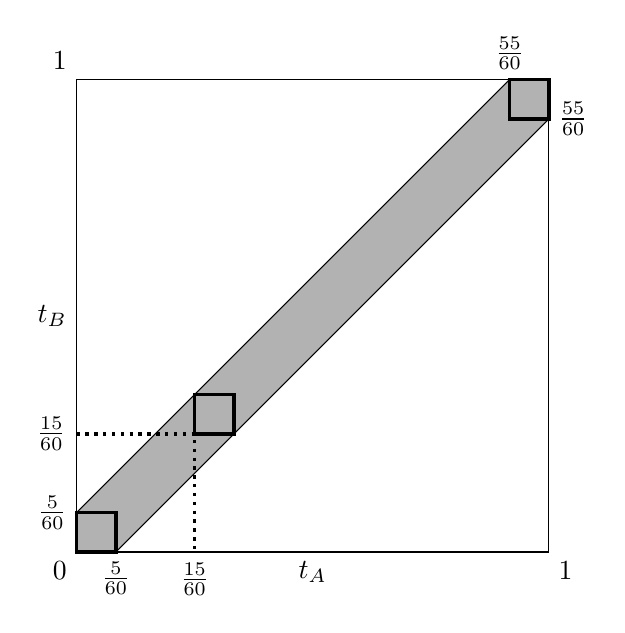
\begin{tikzpicture}
\draw (0,0) -- node[below] {$t_A$} (6,0) -- (6,6) -- (0,6) -- node[left] {$t_B$} cycle;
\node[below left]  at (0,0) {$0$};
\node[below right] at (6,0) {$1$};
\node[above left]  at (0,6) {$1$};
\draw[fill=white!70!black]
  (0,0) -- 
  (.5,0) node[below] {$\frac{5}{60}$} -- 
  (6,5.5) node[right] {$\frac{55}{60}$} --
  (6,6) -- (5.5,6) node[above] {$\frac{55}{60}$} --
  (0,.5) node[left] {$\frac{5}{60}$} -- cycle;
\draw[very thick] (0,0) -- (.5,0) -- (.5,.5) -- (0,.5) -- cycle;
\draw[very thick] (1.5,1.5) -- ++(.5,0) -- ++(0,.5) --
  ++(-.5,0) -- cycle;
\draw[very thick] (5.5,5.5) -- ++(.5,0) -- ++(0,.5) --
  ++(-.5,0) -- cycle;
\draw[very thick,dotted] (0,1.5) node[left] {$\frac{15}{60}$} --
  (1.5,1.5) -- (1.5,0) node[below] {$\frac{15}{60}$};
\end{tikzpicture}
\end{center}
\caption{זמנים המבטיחים מפגש בין $A$ ל-$B$}\label{f.duel}
\end{figure}
אם 
$A$
מגיע יותר מאוחר אזי גם
$B$
חייב להגיע באותו איחור. למשל, אם 
$A$
מגיע ב-%
$t_A=15$,
$B$
חייב להגיע בין
$t_B=15$
ו-%
$t_B=20$.
לכן הפגישה תתקיים בריבוע המתקבל על ידי הזזת הריבוע ב-%
$15$
מ-%
$(0,0)$
ל-%
$(15/60,15/60)$.

ההסתברות לפגישה היא היחס בין השטח האפור בגרף לשטחו של הריבוע הגדול. קל יותר לחשב את המשלים שהוא היחס בין שטח המשולשים הלבנים לשטחו של הריבוע הגדול:
\begin{eqn}
P(\textrm{נפגשים}\;A,B) &=& 1- P(\textrm{נפגשים לא}\;A,B)\\
&=&1- 2\cdot \left(\frac{1}{2}\cdot \frac{55}{60}\cdot \frac{55}{60}\right)=\frac{23}{144}\approx 0.1597\,.
\end{eqn}

\textbf{סימולציה}
\selectlanguage{english}
\begin{verbatim}
Probability of meeting   = 0.1597
Proportion of meetings   = 0.1549
\end{verbatim}
\selectlanguage{hebrew}

%%%%%%%%%%%%%%%%%%%%%%%%%%%%%%%%%%%%%%%%%%%%%%%%%%%%%%%%%%%%%

\begin{prob}{לתפוס את הזייפן הזהיר}{}{(Catching the cautious counterfeiter)}

נתון 
$n$
קופסאות ובכל אחת 
$n$
מטבעות כאשר מטבע אחד בכל קופסה מזויף. שלוף מטבע אחת מכל קופסה ובדוק אם היא מזויפת או אמיתית. מה ההסתברות שכל המטבעות שנשלפות מזויפות?

\que{1} 
פתור עבור
$n=10$.

\que{2} 
פתור עבור 
$n=100$.

\que{3}
פתח נוסחה עבור ההסתברות כאשר
$n$
שרירותי.

\que{4}
פתח נוסחה עבור ההסתברות כאשר
$n$
שואב לאיסוף.
\end{prob}

\solution{}

השליפות בלתי תלויות ולכן ההסתברות שכל המטבעות אמיתיות היא מכפלת ההסתברות עבור שליפה אחת.

\ans{1}
\[
P(\textrm{אמיתיים המטבעות כל}) = \left(\frac{9}{10}\right)^{10}\approx 0.3487\,.
\]


\ans{2}
\[
P(\textrm{אמיתיים המטבעות כל}) = \left(\frac{99}{100}\right)^{100}\approx 0.3660\,.
\]

\ans{3}
\[
P(\textrm{אמיתיים המטבעות כל}) = \left(\frac{n-1}{n}\right)^{n}\,.
\]

\ans{4}
\begin{equation}\label{eq.reciprocal}
\lim_{n\rightarrow\infty}\left(1-\frac{1}{n}\right)^{n}=\frac{1}{e}\,.
\end{equation}

ניתן להוכיח את הגבול באמצעות חשבון דיפרנציאלי. תחילה ניתן לחשב את הגבול של הלוגריתם של הצד השמולי של משוואה%
~\ref{eq.reciprocal}:
\[
\lim_{n\rightarrow\infty}\ln \left(1-\frac{1}{n}\right)^{n}=
  \lim_{n\rightarrow\infty}n\ln \left(1-\frac{1}{n}\right)=
  \lim_{n\rightarrow\infty} \disfrac{\ln\left(1-\frac{1}{n}\right)}{1/n}\,.
\]
אם נחשב את הגבול נקבל
$(\ln \;1)/0=0/0$
אבל לפי חוק
\L{l'H\^{o}pital}
נוכל להחליף את הביטוי בחילוק הנגזרות:
\begin{eqn}
\lim_{n\rightarrow\infty}\ln \left(1-\frac{1}{n}\right)^{n}&=&\lim_{n\rightarrow\infty}\frac{\left(1-\frac{1}{n}\right)^{-1}(-(-n^{-2}))}{-n^{-2}}=-1\\
\lim_{n\rightarrow\infty}\left(1-\frac{1}{n}\right)^{n}&=&e^{-1}\approx 0.3679\,.
\end{eqn}

\textbf{סימולציה}
\selectlanguage{english}
\begin{verbatim}
For  10 boxes:
Probability of all real = 0.3487
Proportion all real     = 0.3480
For 100 boxes:
Probability of all real = 0.3660
Proportion all real     = 0.3730
For 200 boxes:
Probability of all real = 0.3670
Proportion all real     = 0.3690
\end{verbatim}
\selectlanguage{hebrew}

%%%%%%%%%%%%%%%%%%%%%%%%%%%%%%%%%%%%%%%%%%%%%%%%%%%%%%%%%%%%%

\begin{prob}{לתפוס את הזייפן החמדן}{}{(Catching the greedy counterfeiter)}

נתון 
$n$
קופסאות ובכל אחת 
$n$
מטבעות מהן
$m$
מזוייפות. שלוף מטבע אחת מכל קופסה ובדוק אם היא מזויפת או אמיתית. מה ההסתברות 
$P(n,m,r)$
ש-%
$r$
מתוך המטבעות מזוייפות?

\que{1} 
פתח נוסחה עבור
$P(n,m,r)$.

\que{2}
חשב
$P(20,10,2), P(20,10,8), P(20,5,2), P(20,5,4)$.
\end{prob}

\solution{}

\ans{1}
יש 
${n\choose r}$
תת-קבוצות של קבוצת הקופסאות מהן המטבעות המזוייפות נשלפו. לפי ההתפלגות הבינומית:
\[
P(n,m,r) = {n \choose r} \left(\frac{m}{n}\right)^r \left(\frac{n-m}{n}\right)^{n-r}\,.
\]

\ans{2}
\begin{eqn}
P(20,10,2) &=& \dischoose{20}{2} \left(\frac{10}{20}\right)^2 \left(\frac{10}{20}\right)^{18}\approx 0.0002\\
P(20,10,8) &=& \dischoose{20}{8} \left(\frac{10}{20}\right)^{8} \left(\frac{10}{20}\right)^{12}\approx 0.1201\\
P(20,5,2)&=&\dischoose{20}{2} \left(\frac{5}{20}\right)^2 \left(\frac{15}{20}\right)^{18}\approx 0.0669\\
P(20,5,4)&=&\dischoose{20}{4} \left(\frac{5}{20}\right)^{4} \left(\frac{15}{20}\right)^{12}\approx 0.1952\,.
\end{eqn}

\textbf{סימולציה}
\selectlanguage{english}
\begin{verbatim}
For 10 bad coins,  2 draws:
Probability of counterfeit  = 0.0002
Proportion counterfeit      = 0.0002
For 10 bad coins,  8 draws:
Probability of counterfeit  = 0.1201
Proportion counterfeit      = 0.1181
For  5 bad coins,  2 draws:
Probability of counterfeit  = 0.0669
Proportion counterfeit      = 0.0688
For  5 bad coins,  4 draws:
Probability of counterfeit  = 0.1897
Proportion counterfeit      = 0.1905
\end{verbatim}
\selectlanguage{hebrew}

\L{Mosteller}
משתמש בגבול מבעיה 
$27$
כדי להראות שעבור 
$m,r$
נתון, כאשר 
$n$
שואף לאינסוף:
\begin{equation}\label{eq.bin-limit}
\lim_{n\rightarrow \infty}P(n,m,r) = \frac{e^{-m}m^r}{r!}\,.
\end{equation}
הנה השוואה של ההסתברויות עבור 
$m=10, r=8$
עבור ערכים עולים של
$n$:
\selectlanguage{english}
\begin{verbatim}
Limit = 0.11259903, binomial = 0.11482303, n = 100
Limit = 0.11259903, binomial = 0.11282407, n = 1000
Limit = 0.11259903, binomial = 0.11262155, n = 10000
Limit = 0.11259903, binomial = 0.11259926, n = 1000000
\end{verbatim}
\selectlanguage{hebrew}

%%%%%%%%%%%%%%%%%%%%%%%%%%%%%%%%%%%%%%%%%%%%%%%%%%%%%%%%%%%%%

\begin{prob}{\protect עובש בג'לטין}{}{(Moldy gelatin)}

נתון לוח מלבני שמחולק ל-%
$n$
משבצות ריבועיות קטנות. בכל משבצת יש 
$r$ 
חיידקים בממוצע.

\que{1} 
פתח נוסחה להסתברות שיש בדיוק 
$r$
חיידקים ב-%
$n$
המשבצות.

\que{2}
חשב את ההסתברות עבור
$n=100,r=3$.

\textbf{רמז:}
בעיה זו דומה לבעיה%
~$28$.

\end{prob}

\solution{}

\ans{1}
$p$,
ההסתברות שבמשבצת אחת נמצא חידק (נתעלם מהאפשרות שחיידק אחד מוכל באופן חלקי בשתי משבצות או יותר), היא
$m/n$.
$P(n,m,r)$,
ההסתברות שיש בדיוק 
$r$
חיידקים ב-%
$n$
משבצות' ניתנת על ידי ההתפלגות הבינומית:
\[
P(n,m,r) = {n \choose r} \left(\frac{m}{n}\right)^r \left(\frac{n-m}{n}\right)^{n-r}\,.
\]

\ans{2} 
\[
P(10,3,3) = {100 \choose 3} \left(\frac{3}{100}\right)^3 \left(\frac{97}{100}\right)^{97}\approx 0.2275\,.
\]

\textbf{סימולציה}
\selectlanguage{english}
\begin{verbatim}
For  20 squares:
Probability of exactly  3 microbes  = 0.2428
Proportion of exactly   3 microbes  = 0.2436
Probability of exactly  5 microbes  = 0.2023
Proportion of exactly   5 microbes  = 0.1954
For 100 squares:
Probability of exactly  3 microbes  = 0.2275
Proportion of exactly   3 microbes  = 0.2247
Probability of exactly  5 microbes  = 0.1800
Proportion of exactly   5 microbes  = 0.1851
\end{verbatim}
\selectlanguage{hebrew}


משוואה%
~\ref{eq.bin-limit}
מתאים גם כאן לחשב את הגבול כאשר 
$n$
שואף לאינסוף:
\begin{eqnarray*}
\lim_{n\rightarrow \infty}P(n,m,r) &=& \frac{e^{-m}m^r}{r!}\\
\lim_{n\rightarrow \infty} P(n,3,3) &=& \frac{e^{-3}\cdot 3^3}{3!}\approx 0.2240\\
\lim_{n\rightarrow \infty} P(n,5,5) &=& \frac{e^{-5}\cdot 5^5}{5!}\approx 0.1755\,.
\end{eqnarray*}

%%%%%%%%%%%%%%%%%%%%%%%%%%%%%%%%%%%%%%%%%%%%%%%%%%%%%%%%%%%%%

\refstepcounter{problem} % 30. Evening the sales

%%%%%%%%%%%%%%%%%%%%%%%%%%%%%%%%%%%%%%%%%%%%%%%%%%%%%%%%%%%%%

\begin{prob}{ימי הולדת זהים}{}{(Birthday pairings)}

\que{1}
עבור 
$n$
אנשים מה ההסתברות 
$P(n)$
שלניים מהם או יותר יש יום הולדת זהה?

\que{2}
מה מערך הקטן ביותר עבור 
$n$
כך ש-%
$P(n)>0.5$?

הנח שההתפלגות של ימי ההודלת היא אחידה בטווח
$[1,365]$.

\textbf{רמז:}
חשב את המשלים להסתברות של-%
$n$
אנשים ימי הולדת 
\textbf{שונים}.
\end{prob}

\solution{}

\ans{1}
בחר 
$n$
אנשים אחד אחרי השני ובדוק אם יש להם אותו יום הולדת כמו הקודמים שנבחרו. עבור הראשון יש 
$365$
ימים, עבור השני
$364$
ימים וכך הלאה:
\[
1-P(n)=
  \overbrace{\disfrac{365}{365}\cdot\frac{364}{365}
  \cdot \;\cdots \; \cdot \frac{365-(n-2)}{365}
  \cdot\frac{365-(n-1)}{365}}^{n}
=\disfrac{365!/(365-n)!}{365^{n}}\,.
\]

\ans{2}
חשב ערך זה עבור ערכים שונים של
$n$
או השתמש בתכנית מחשב כדי לחפש מ-%
$1$
ל-%
$365$
כדי למצוא את הערך הראשון עבורו
$1-P(n)<0.5$.
הערך הוא
$23$:
\[
1-P(23)=\disfrac{365!}{365^{23}\cdot 342!}\approx 0.4927\,.
\]
רוב האנשים מופתעים שהתשובה היא ערך כל קטן.

מחשבון מודרני מסוגל לחשב 
$1-P(n)$
אבל שווה לחשב אותו באמצעות הקירוב של 
\L{Stirling}
שהוא
$\ln n! \approx n\ln n - n$:
\begin{eqnarray*}
\ln (1-P(n))&=&
  \ln\left(\disfrac{365!}{342!\cdot 365^{23}}\right)=\ln 365! - \ln 342! -23 \ln 365\\
&\approx& (365\ln 365 -365) - (342\ln 342 -342) - 23\,\ln 365 \\
&\approx&-0.7404\\
1-P(n)&\approx&e^{-0.7404}=0.4769\,.
\end{eqnarray*}
הקורא מוזמן לחשב את ההסתברות עם הקירוב המדוייק יותר:
\[
\ln n!  \approx n\ln n - n + \frac{1}{6}\left(8n^3+4n^2+n+\frac{1}{30}\right)+\frac{1}{2}\ln\pi\,.
\]
\textbf{סימולציה}
\selectlanguage{english}
\begin{verbatim}
For 21 people:
Expectation of no pairs = 0.5563
Average no pairs        = 0.5497
For 22 people:
Expectation of no pairs = 0.5243
Average no pairs        = 0.5237
For 23 people:
Expectation of no pairs = 0.4927
Average no pairs        = 0.4933
For 24 people:
Expectation of no pairs = 0.4617
Average no pairs        = 0.4576
For 25 people:
Expectation of no pairs = 0.4313
Average no pairs        = 0.4345
\end{verbatim}
\selectlanguage{hebrew}

%%%%%%%%%%%%%%%%%%%%%%%%%%%%%%%%%%%%%%%%%%%%%%%%%%%%%%%%%%%%%

\begin{prob}{למצוא עמית ליום הולדת}{}{(Finding your birthmate)}

\textbf{עמית ליום הולדת},
בקיצור עמית, הוא אדם עם יום הולדת זהה לשלך.

מדוע מציאת עמית היא בעיה שונה ממציאת זוג עם ימי הולדת זהים?

\que{1}
כמה אנשים עליך לשאול עד ש-%
$Q(n)$,
ההסתברות למציאת עמית, גבוהה מ-%
$0.5$?

\que{2}
פתור את הבעיה על ידי שימוש במשוואה%
~\ref{eq.reciprocal}.
\end{prob}

\solution{}

להרבה אנשים יכול להיות יום הולדת זהה שנחשב כהצלחה במציאת זוג, אבל לא הצלחה במציאת עמית אלא אם יום ההולדת של האדם האחר זהה לשלך.

\ans{1}
נמצא את
$n$,
המספר הקטן ביותר של אנשים, כך ש-%
$1-Q(n)$,
ההסתברות שלאף אחד מהם הוא לא עמית, פחות מ-%
$0.5$.
ההסתברות שהאדם הראשון שאתה שואל אינו עמית היא
$364/365$,
אבל זאת גם ההסתברות שהשני, השלילי, 
\ldots, 
אינו עמית. הפתרון הוא ה-%
$k$
הקטן ביותר כך ש:
\[
1-Q(n)=\left(\frac{364}{365}\right)^n<\frac{1}{2}\,.
\]
בחיפוש עם מחשב נמצא ש-%
$n=253$:
\[
\left(\frac{364}{365}\right)^{253} \approx 0.4995\,.
\]
\ans{2}
משוואה%
~\ref{eq.reciprocal}
היא:
\[
\lim_{n\rightarrow\infty}\left(\frac{n-1}{n}\right)^{n}=\frac{1}{e}\,,
\]
וניתן להשתמש בה לחשב את ההסתברות:
\begin{eqn}
1-Q(n)&=&
  \left(\disfrac{365-1}{365}\right)^n=\left[\left(\disfrac{364}{365}\right)^{365}\right]^{n/365}\\
&\approx& e^{-n/365}\\
e^{-253/365}&\approx&0.5000\,.
\end{eqn}

\newpage

\textbf{סימולציה}
\selectlanguage{english}
\begin{verbatim}
For 251 people:
Probability of no match = 0.5023
Proportion no match     = 0.5120
For 252 people:
Probability of no match = 0.5009
Proportion no match     = 0.5055
For 253 people:
Probability of no match = 0.4995
Proportion no match     = 0.4984
For 254 people:
Probability of no match = 0.4982
Proportion no match     = 0.4987
For 255 people:
Probability of no match = 0.4968
Proportion no match     = 0.5078
\end{verbatim}
\selectlanguage{hebrew}

%%%%%%%%%%%%%%%%%%%%%%%%%%%%%%%%%%%%%%%%%%%%%%%%%%%%%%%%%%%%%

\begin{prob}{השוואת הבעיית יום הולדת זהה לבעיית עמית ליום הולדת}{}{\\(Relating the birthday pairings and the birthmate problems)}

סמן ב-%
$P(r)$
את ההסתברות למצוא זוג שלהם ימי הולדת זהים מתוך
$r$
אנשים (בעיה~$31$), וב-%
$Q(n)$
את ההסתברות שמתוך
$n$
אנשים לפחות אחד הוא עימית שלך (בעיה~$32$).
נתון
$r$
עבור איזה
$n$,
$P(r) \approx Q(n)$?
\end{prob}

\solution{1}

הפתרון מבוסס על
\L{\cite{birthday}}.

מהפתרון לבעיית%
~$31$
מתקבל:
\[
\renewcommand*{\arraystretch}{2.2}
\begin{array}{lcl}
P(r)&=&
\disfrac{365}{365}\cdot 
  \frac{365-1}{365}\cdot \frac{365-2}{365} \cdot\;
  \cdots \;\cdot \frac{365-(r-1)}{365}\\
&=&1\left(1-\disfrac{1}{365}\right)
  \left(1-\disfrac{2}{365}\right) \cdot\;
  \cdots \;\cdot \left(1-\disfrac{r-1}{365}\right)\\
&\approx&1-\disfrac{1}{365} - \disfrac{2}{365} -
  \cdots - \disfrac{r-1}{365}\\
&=&1-\disfrac{1+2+3+\cdots + (r-1)}{365}\\
&=&1-\disfrac{r(r-1)/2}{365}\,,
\end{array}
\]
כאשר הקירוב במשוואה השלישית מתקבל מהשמטת חזקות של
$1/365$
גדולות מאחת כי הן קטנות מדי להשפיע באופן מהותי על התוצאה.

באמצעות באותו קירוב, מהפתרון לבעיה%
~$32$
מתקבל:
\[
\renewcommand*{\arraystretch}{2.2}
\begin{array}{lcl}
P_{\textrm{\footnotesize עמית אין}}(n)
&=&\overbrace{\left(1-\frac{1}{365}\right)
  \left(1-\frac{1}{365}\right)\cdots
  \left(1-\frac{1}{365}\right)}^{n}\\
&\approx& 1-\overbrace{\frac{1}{365}-\frac{1}{365}\cdots-
  \frac{1}{365}}^{n}\\
&\approx& 1-\disfrac{n}{365}\\
\end{array}
\]
לכן
$P(r)\approx Q(n)$
כאשר:
\[
n=\frac{r(r-1)}{2}\,.
\]
עבור
$r=23$, $n=(23\cdot 22)/2=253$.

\solution{2}

\L{Mosteller}
מביא את הפתרון האיטואיטיבי שלהלן:
\begin{quote}
כאשר משווים בין בעיית הזוג והעמית, אנו שמים לב שעבור 
$r$
אנשים בבעיית הזוג, קיימים 
$r(r-1)/2$
זוגות או 
\textbf{הזדמנויות}
לידי הולדת זהים; לעומת זאת, אם שואלים 
$n$
אנשים בבעיית העמית קיימות רק 
$n$
הזדמנויות כדי שאמצא עמית אחד או יותר
\L{\cite[p.~322]{birthday}}.
\end{quote}
מכאן הוא מסיק ש-%
$n\approx r(r-1)/2$.

ניתן להבין את הטיעון כך: בבעיית הזוג בחר תאריך שרירותי ושאל אם לשניים מתוך
$r$
\textbf{תאריך זה}
הוא יום ההולדת שלהם. יש:
\[
{r \choose 2}=\frac{r!}{2!(r-2)!} = \frac{r(r-1)}{2}
\]
דרכים שזה אפשרי. עבור בעיית העמית יום ההולדת שלך נתון, ולכל אחד מתוך
$n$
אנשים יש אותו סיכוי ליום הולדת זהה. על ידי השוואת שני הביטוים נקבל 
$n$
עבורו
$P_(r) \approx Q(n)$.

\textbf{סימולציה}

תוכל להריץ את הסימולציות לבעיות
~$31, 32$
ולבדוק תוצאה זו.

%%%%%%%%%%%%%%%%%%%%%%%%%%%%%%%%%%%%%%%%%%%%%%%%%%%%%%%%%%%%%

\begin{prob}{חופש בימי הולדת}{D}{(Birthday holidays)}

בית חרושת נסגר בכל יום שהוא יום הולדת של אחד העובדים. אין חופשות נוספות.

\que{1} 
כמה עובדים כדאי להעסיק כדי למקסם את מספר ימי-העבודה בשנה אחת?

\que{2}
מה התוחלת של היחס בין מספר ימי-העבודה המקסימליים לבין
$365^2$, 
מספר ימי-העבודה עם כל אחד מ-%
$365$
העובדים עובדים כל יום?

\textbf{רמז:}
הוכח על ידי בדיקת מקרי הקצה שמקסימום חייב להתקיים. אחר כך פתח נוסחה של התוחלת של ימי-העבודה ביום אחד.
\end{prob}

\solution{}

\ans{1}
אם יש רק עובד אחד יהיו 
$364$
ימי-עבודה. אם יש שני עובדים מספר ימי-העבודה הוא
$363+363=726$
(כאשר נתעלם המאפשרות הזניחה שלשניהם אותו יום הולדת). בקצה השני אם יש מיליון עובדים מספר ימי-העבודה יהיה אפס כמעט בוודאות. אם מספר ימי-העבודה עולה ואחר כך חוזר לאפס, חייב להיות מקסימום בין נקודות הקצה.

כדי לפשט את הסימונים נסמן את המספר הימים בשנה ב-%
$N$
ומספר העובדים ב-%
$n$.

יהי
$p=\disfrac{N-1}{N}=1-\disfrac{1}{N}$. 
ההסתברות שיום נתון הוא יום-עבודה היא ההסתברות שלכל עובד יום הולדת בתאריך אחר:
\[
\overbrace{\disfrac{N-1}{N} \cdot \;\cdots\;\cdot \disfrac{N-1}{N}}^n = \left(1-\disfrac{1}{N}\right)^n=p^n\,.
\]
ביום עבודה כל העובדים עובדים וביום חופש אף אחד לא עובד ולכן:
\[
E(\textrm{נתון ליום ימי-עבודה}) = n \cdot p^n + 0\cdot (1-p^n) = np^n\,.
\]
לכל ימי השנה אותה תוחלת ולכן:
\begin{equation}\label{eq.holidays}
E(\textrm{לשנה ימי-עבודה}) = Nnp^n\,.
\end{equation}
כדי למצוא את המקסימום נגזור את משוואה%
~\ref{eq.holidays}
ביחס ל-%
$n$
ונשמתש ב-%
$(p^n)'=p^n\ln p$
ניתן להוכיח בעזרת חוק השרשרת:
\[
(p^n)' = ((e^{\ln p})^n)' =
(e^{n\ln p})' =
e^{n\ln p} (n\ln p)'=
(e^{\ln p})^n \ln p = p^n\ln p\,.
\]
הנגזרת של משוואה%
~\ref{eq.holidays}
היא:
\[
(Nnp^n)'= N (p^n + n (p^n)') = N (p^n + np^n\ln p)\,,
\]
שהיא $0$ כאשר:
\[
n=-\disfrac{1}{\ln p}\,.
\]
עבור
$N=365$
מתקבל
$n=364.5$
אבל
$n$
הוא מספר שלם ולכן המקסימום מתקבל ב-%
$n=364$
או
$n=365$
שנותנים אותו תוחלת של ימי-עבודה:
\begin{eqn}
E(\textrm{לשנה ימי-עבודה}) &=&Nnp^n\\
&=&365\cdot 364 \cdot \left(\disfrac{364}{365}\right)^{364}\\
&=&365\cdot 364  \cdot \disfrac{365}{365}\left(\disfrac{364}{365}\right)^{364}\\
&=&365\cdot 365  \cdot \left(\disfrac{364}{365}\right)^{365}\\
&=&48944\,.
\end{eqn}

\ans{2}
התוחלת של היחס היא:
\[
E(\textrm{מקסימליים ימי-עבודה}/\textrm{אפשריים ימי-עבודה})
=\disfrac{365\cdot 365  \cdot \left(\frac{364}{365}\right)^{365}}{365\cdot 365}=\left(\disfrac{364}{365}\right)^{365}\approx 0.3674\,.
\]
לפי משוואה%
~\ref{eq.reciprocal}:
\[
\lim_{n\rightarrow\infty}
E(\textrm{מקסימליים ימי-עבודה}/\textrm{אפשריים ימי-עבודה})
=\lim_{N\rightarrow \infty} \left(1-\disfrac{1}{N}\right)^N= \disfrac{1}{e}\,.
\]

\textbf{סימולציה}
\selectlanguage{english}
\begin{verbatim}
For 100 people
Expectation work-days    =  27742
Average work days        =  27743
Ratio work-days / 365**2 = 0.2082
For 250 people
Expectation work-days    =  45958
Average work days        =  45939
Ratio work-days / 365**2 = 0.3450
For 364 people
Expectation work-days    =  48944
Average work days        =  48936
Ratio work-days / 365**2 = 0.3674
For 365 people
Expectation work-days    =  48944
Average work days        =  48917
Ratio work-days / 365**2 = 0.3674
\end{verbatim}
\selectlanguage{hebrew}

%%%%%%%%%%%%%%%%%%%%%%%%%%%%%%%%%%%%%%%%%%%%%%%%%%%%%%%%%%%%%

\begin{prob}{על שפת התהום}{}{(The cliff-hanger)}

חלקיק מוצב על ציר ה-%
$x$
במקום
$1$.
בכל מקום על ציר ה-%
$x$
הוא יכול לצעוד צעד ימינה עם הסתברות
$2/3$
וצעד שמאלה עם הסתברות
$1/3$
(איור%
~\ref{f.ruin1}).

\que{1}
מה ההסתברות שהחלקיק יגיע למקום
$0$
בסופו של דבר?

\que{2}
אם ההסתברות של צעד ימינה היא
$p$
וההסתברות של צעד שמאלה היא
$1-p$,
מה ההסתברות שהחלקיק יגיע למקום
$0$
בסופו של דבר? נתח את האפשרויות לערכים שונים של
$p$.

\textbf{רמז:}
השתשמש בהסתרויות מותנות לאחר הצעד הראשון.
\begin{figure}[tb]
\begin{center}
\begin{tikzpicture}[scale=1.5]
\draw (0,0) -- (6,0);
\draw[dashed] (6,0) -- (8,0) node[right] {$\infty$};
\foreach \x in {0,1,2,3,4,5,6} {
  \draw (\x,0) -- +(0,4pt);
  \node at (\x,-10pt) { $\x$ };
}
\draw[fill] (1,5mm) circle[radius=.5pt];
\draw[->] (1,5mm) -- node[above] {$1/3$} (0,5mm);
\draw[->,very thick] (1,5mm) -- node[above] {$2/3$} (2,5mm);

\foreach \x/\y in {2/10mm,3/15mm,4/20mm} {
  \draw[fill] (\x,\y) circle[radius=.5pt];
  \draw[->] (\x,\y) -- node[above] {$1/3$} (\x-1,\y);
  \draw[->] (\x,\y) -- node[above] {$2/3$} (\x+1,\y);
}
\end{tikzpicture}
\end{center}
\caption{?האם חלקיק יכול להגיע ל-$0$ (הציר אינסופי לימין)}\label{f.ruin1}
\end{figure}
\end{prob}

\newpage

\solution{}

\ans{1,2}
נסמן צעד שמאלה ב-%
$L$
וצעד ימינה ב-%
$R$.
החלקיק יכול להגיע ל-%
$0$
ישירות על ידי צעד
$L$
עם הסתברות
$\frac{1}{3}$,
או על ידי צעד
$RLL$
עם הסתברות
$\frac{2}{3}\cdot\frac{1}{3}\cdot\frac{1}{3}$,
או על ידי צעד
$RRLLL$
עם הסתברות
$\left(\frac{2}{3}\right)^2\left(\frac{1}{3}\right)^3$, \ldots\ .
החישוב נראה כמו סידרה הנדסית פשוטה אבל הוא מתעלם האפשרויות כגון
$RLRLL$.

נסמן ב-%
$P(i,j)$
את ההסתברות שהחלקיק מגיע ל-%
$i$
מ-%
$j$.
נחשב את ההתסתברות שהחלקיק מגיעה ל-%
$0$
מ-%
$1$
כתלות בצעד הראשון:
\begin{eqn}
P(0,1) &=& 
P(0,1|\textrm{שמאלה ראשון צעד}) + P(0,1|\textrm{ימינה ראשון צעד})\\
&=& (1-p)\cdot 1 + pP(1,2)P(0,1)\,.
\end{eqn}
אבל
$P(1,2) = P(0,1)$
ומתקבלת משוואה ריבועית ב-%
$P(0,1)$:
\begin{eqn}
P(0,1) &=& (1-p) + pP(0,1)^2\\
pP^2(0,1) - P(0,1) + (1-p) &=&0\\
%P(0,1)&=& \frac{1\pm\sqrt{1-4p(1-p)}}{2p}\\
P(0,1)&=&1,\; (1-p)/p\,.
\end{eqn}
אם
$p\leq 1/2$
אזי
$(1-p)/p\geq 1$, 
כך ש-%
$P=1$
הוא הפתרון היחיד ובטוח שהחלקיק יגיע ל-%
$0$.

אם 
$p=1$
אזי
$P=0$
כי אם החלקיק תמיד צועד ימינה הוא לא יכול להחזור ל-%
$0$.

נניח ש-%
$P(0,1)=1$
עבור
$1/2<p < 1$,
כלומר,
$P(0,1)$
\textbf{לא תלוי ב-}$p$.
באיור%
~\ref{f.ruin2}
הקו האדום המקווקוו האדום מראה את עבור
$P(1,0)$
כאשר 
$p$
שואף ל-%
$1$
והנקודה האדומה מראה ש-%
$P(1,0)=0$
כאשר 
$p$
מגיע ל-%
$1$.
$P(0,1)$
לא יכולה פתאום "לקפוץ" מ-%
$1$
ל-%
$0$
ולכן עבור
$p> 1/2$
הפתרון היחיד הוא
$P=(1-p)/p< 1$.\footnote{\L{Mosteller}
כותב שזה נובע מרציפות אבל הוא לא נותן הוכחה.}

\begin{figure}[tb]
\begin{center}
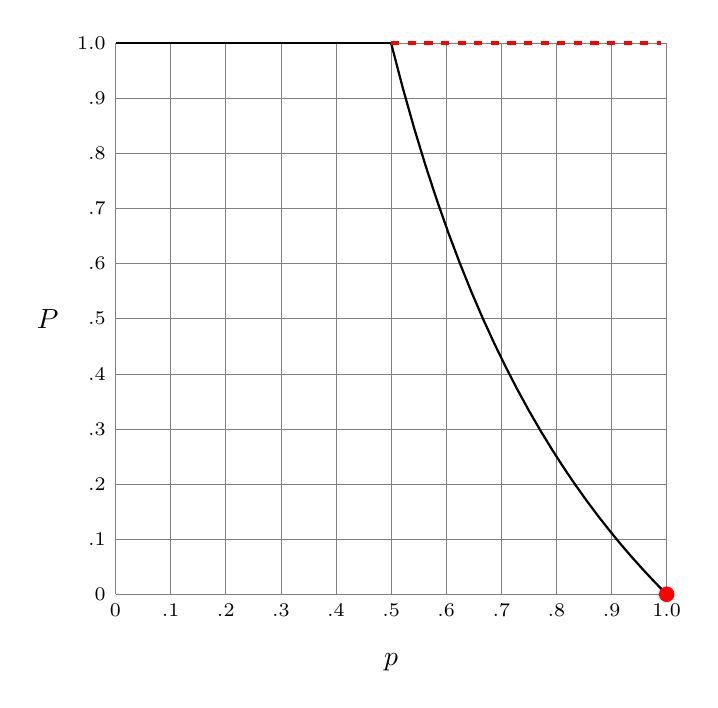
\begin{tikzpicture}[scale=7]
\draw[help lines,step=.1] (0,0) grid (1,1);
\foreach \x in {0,.1,.2,.3,.4,.5,.6,.7,.8,.9,1.0}
  \node[below] at (\x,0) {$\scriptstyle \x$};
\foreach \y in {0,.1,.2,.3,.4,.5,.6,.7,.8,.9,1.0}
  \node[left] at (0,\y) {$\scriptstyle \y$};
\draw[domain=0:.5,thick] plot (\x,1);
\draw[domain=.5:1,thick] plot (\x,{(1-\x)/\x});
\node at (.5,-3.5pt) {$p$};
\node at (-3.5pt,.5) {$P$};
\draw[ultra thick,red,dashed] (.5,1) -- +(.49,0);
\fill[red] (1,0) circle[radius=.4pt];
\end{tikzpicture}
\end{center}
\caption{הגרף של $P=\min(p/(1-p),1)$ עבור $p\in [0,1]$}\label{f.ruin2}
\end{figure}
עבור
$p=2/3, P=1/2$
ועבור
$p=1/2, P=1$.
זה מפתיע כי לא היינו מצפים שהחלקיק יחזור תמיד ל-%
$0$
אם כיוון הצעד נקבע על ידי הטלת מטבע הוגן! אנו זקוקים למטבע ממש לא-הוגן (הסתברות של "עץ" שווה ל-%
$2/3$)
כדי להשוות את הסיכויים לחזור ל-%
$0$
או לא.

\newpage

\textbf{סימולציה}
\selectlanguage{english}
\begin{verbatim}
For probability = 0.2500:
Probability of reaching 0 = 1.0000
Proportion reaching 0     = 1.0000
For probability = 0.5000:
Probability of reaching 0 = 1.0000
Proportion reaching 0     = 0.9612
For probability = 0.6667:
Probability of reaching 0 = 0.5000
Proportion reaching 0     = 0.5043
For probability = 0.7500:
Probability of reaching 0 = 0.3333
Proportion reaching 0     = 0.3316
For probability = 0.8000:
Probability of reaching 0 = 0.2500
Proportion reaching 0     = 0.2502
\end{verbatim}
\selectlanguage{hebrew}

%%%%%%%%%%%%%%%%%%%%%%%%%%%%%%%%%%%%%%%%%%%%%%%%%%%%%%%%%%%%%

\begin{prob}{פשיטת הרגל של מהמר}{D}{(Gambler's ruin)}

חלקיק מוצב על ציר ה-%
$x$
במקום
$m\geq 1$.
בכל מקום על ציר ה-%
$x$
הוא יכול לצעוד צעד ימינה עם הסתברות
$p>1/2$
וצעד שמאלה עם הסתברות
$1-p$.

\que{1}
מה ההסתברות שהחלקיק יגיע למקום
$0$
בסופו של דבר?

\que{2} יהי 
$n>m$.
אם החלקיק מגיע למקום 
$0$
או למקום
$n$
הוא מפסיק לצעוד (איור%
~\ref{f.ruin3}).
מה ההסתברות שהחלקיק יגיע למקום 
$0$?
מה ההסתברות שהחלקיק יגיע למקום
$n$?
\begin{figure}[tb]
\begin{center}
\begin{tikzpicture}[scale=1.5]
\draw (0,0) -- (6,0);
\foreach \x in {0,1,2,3,4,5,6} {
  \draw (\x,0) -- +(0,4pt);
  \node at (\x,-10pt) { $\x$ };
}
\node at (2,-20pt) {$m$};
\node at (6,-20pt) {$n$};
\draw[fill] (2,5mm) circle[radius=.5pt];
\draw[->] (2,5mm) -- node[above] {$1/3$} (1,5mm);
\draw[->] (2,5mm) -- node[above] {$2/3$} (3,5mm);
\end{tikzpicture}
\end{center}
\caption{האם החלקיק יכול לחזור ל-%
$0$ (ציר סופי)?}
\label{f.ruin3}
\end{figure}

\textbf{הערה:} 
בעיה%
~$35$
מייצגת מהמר המשחק עם כמות סופית של כסף נגד קזינו עם כמות בלתי מוגבלת של כסף. הבעיה מבקשת את ההסתברות שהמהמר יפסיד את כל כספו. בעיה~%
$36(2)$
שואלת על מהמר אחד עם 
$m$
שמשחק נגד מהמר שני עם 
$n-m$.
הבעיה מבקשת את ההסתברויות ש%
\textbf{אחד}
מהם מפסיד את כל כספו לשני.
\end{prob}

\solution{}

הפתרון מבוסס על
\L{\cite[Chapter~2, Example~4m]{ross}}.

נסמן ב-%
$P(i,j)$
את ההסתברות שהחלקיק מגיע ל-%
$i$
מ-%
$j$.

\ans{1}
ראינו בפתרון לבעיה%
~$35$
שעבור
$p>1/2$
(כאן נתון), אם חלקיק נמצא במקום 
$1$
ההסתברות שלו להגיע ל-%
$0$
היא
$r=(1-p)/p$.
הסתברות זו לא תלויה במקום האבסולוטי של החלקיק ולכן:
\[
P(i,j) = P(i+k,k+1) = P(i-k,j-k)\,,
\]
ו-%
\begin{equation}
P(0,m)=P(m-1,m)P(m-2,m-1)\cdots P(1,2)P(0,1)=r^m\,.
\end{equation}

\ans{2} 
סמן בקיצור
$P_i=P(n,i)$
וחשב את
$P_i$:
\begin{eqn}
P_i &=& pP_{i+1} + (1-p)P_{i-1}\\
%pP_{i+1}&=&1\cdot P_i - (1-p)P_{i-1}\\
pP_{i+1}&=&(p+(1-p))P_i - (1-p)P_{i-1}\\
p(P_{i+1}-P_i)&=&(1-p)(P_i-P_{i-1})\\
P_{i+1}-P_i&=&r(P_i-P_{i-1})\,.
\end{eqn}
$P_0=0$ 
כי אם החלקיק נמצא ב-%
$0$
הוא מפסיק לצעוד. לכן:
\begin{eqn}
P_2 - P_1 &=& r(P_1 - P_0) = rP_1\\
P_3 - P_2 &=& r(P_2 - P_1) = r^2P_1\\
\cdots &=&\cdots\\
P_i - P_{i-1} &=& r(P_{i-1} - P_{i-2}) = r^{i-1}P_1\,.
\end{eqn}
רוב הגורמים בצד השמאלי מצטמצמים כאשר מחברים את המשוואות:
\begin{eqnlabels}
\nonumber{}P_i - P_1 &=& P_1\sum_{j=2}^{i}r^{j-1}\\
\nonumber{}&=& P_1 + P_1\sum_{j=2}^{i}r^{j-1} - P_1 \\
\label{eq.ruin0}P_i&=& P_1\sum_{j=0}^{i-1}r^j =P_1\left(\frac{1-r^i}{1-r}\right)\,.
\end{eqnlabels}
אם חלקיק נמצא ב-%
$n$
הוא כבר נמצא ב-%
$n$
כך ש-%
$P_n=1$:
\begin{eqnlabels}
\nonumber{}1 &=& P_1\left(\frac{1-r^n}{1-r}\right)\\
\label{eq.ruin00}P_1 &=& \left(\frac{1-r}{1-r^n}\right)\,.
\end{eqnlabels}
ממשוואות%
~\ref{eq.ruin0}, \ref{eq.ruin00}:
\begin{equation}
\label{eq.ruin1}P(n,i) = \left(\frac{1-r^{i}}{1-r^n}\right)\,.
\end{equation}
בהוכחה סימטרית שמחליפה את
$p$
ו-%
$1-p$):
\begin{equation}
\label{eq.ruin2}P(0,i) = \left(\frac{1-(1/r)^{n-i}}{1-(1/r)^{n}}\right)\,.
\end{equation}
הקורא מוזמן להראות שהסכום של משוואות
~\ref{eq.ruin1},~\ref{eq.ruin2}
הוא $1$ כלומר שמובטח שאחד המהמרים ינצח והשני יפסיד. עבור
$m=1, n=3, p=2/3$:
\begin{eqn}
P(0,1) &=& \left(\frac{1-\left(\frac{1}{2}\right)^{1}}{1-\left(\frac{1}{2}\right)^{3}}\right)=\frac{4}{7}\\
P(3,1) &=& \left(\frac{1-2^{2}}{1-2^{3}}\right)=\frac{3}{7}\,.
\end{eqn}

\textbf{סימולציה}
\selectlanguage{english}
\begin{verbatim}
For probability = 0.6667:
Probability of reaching (0,10) from 1 = (0.4995,0.5005)
Proportion reaching     (0,10) from 1 = (0.5056,0.4944)
Probability of reaching (0,10) from 4 = (0.0616,0.9384)
Proportion reaching     (0,10) from 4 = (0.0643,0.9357)
Probability of reaching (0,10) from 6 = (0.0147,0.9853)
Proportion reaching     (0,10) from 6 = (0.0123,0.9877)
\end{verbatim}

\begin{verbatim}
For probability = 0.7500:
Probability of reaching (0,10) from 1 = (0.3333,0.6667)
Proportion reaching     (0,10) from 1 = (0.3395,0.6605)
Probability of reaching (0,10) from 4 = (0.0123,0.9877)
Proportion reaching     (0,10) from 4 = (0.0115,0.9885)
Probability of reaching (0,10) from 6 = (0.0014,0.9986)
Proportion reaching     (0,10) from 6 = (0.0015,0.9985)
\end{verbatim}
\selectlanguage{hebrew}
ככל שלמהמר בצד שמאל יש יותר והסתברות גבוהה היותר לזכות בכל צעד, כך ההסתברות שלו לניצחון גדלה.

\textbf{גרף של הצעדים}

הגרף נוצר בעזרת ספריית 
\L{\texttt{matplotlib}}
של
\L{Python}.
קור המקור מופיע בקובץ:
\begin{center}
\L{\texttt{36-gamblers-ruin-plot.py}}
\end{center}
\begin{center}
% This file was created with tikzplotlib v0.10.1.
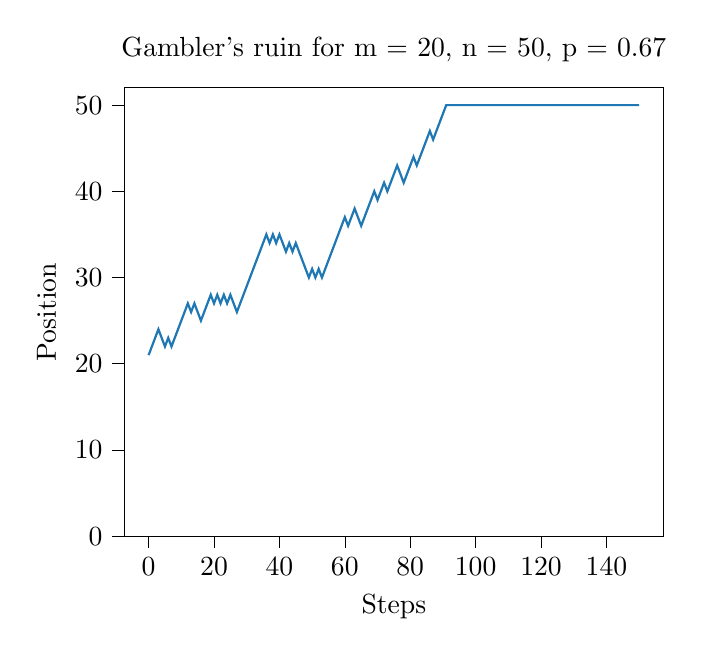
\begin{tikzpicture}

\definecolor{darkgray176}{RGB}{176,176,176}
\definecolor{steelblue31119180}{RGB}{31,119,180}

\begin{axis}[
tick align=outside,
tick pos=left,
title={Gambler's ruin for m = 20, n = 50, p = 0.67},
x grid style={darkgray176},
xlabel={Steps},
xmin=-7.5, xmax=157.5,
xtick style={color=black},
y grid style={darkgray176},
ylabel={Position},
ymin=0, ymax=52,
ytick style={color=black}
]
\addplot [thick, steelblue31119180]
table {%
0 21
1 22
2 23
3 24
4 23
5 22
6 23
7 22
8 23
9 24
10 25
11 26
12 27
13 26
14 27
15 26
16 25
17 26
18 27
19 28
20 27
21 28
22 27
23 28
24 27
25 28
26 27
27 26
28 27
29 28
30 29
31 30
32 31
33 32
34 33
35 34
36 35
37 34
38 35
39 34
40 35
41 34
42 33
43 34
44 33
45 34
46 33
47 32
48 31
49 30
50 31
51 30
52 31
53 30
54 31
55 32
56 33
57 34
58 35
59 36
60 37
61 36
62 37
63 38
64 37
65 36
66 37
67 38
68 39
69 40
70 39
71 40
72 41
73 40
74 41
75 42
76 43
77 42
78 41
79 42
80 43
81 44
82 43
83 44
84 45
85 46
86 47
87 46
88 47
89 48
90 49
91 50
92 50
93 50
94 50
95 50
96 50
97 50
98 50
99 50
100 50
101 50
102 50
103 50
104 50
105 50
106 50
107 50
108 50
109 50
110 50
111 50
112 50
113 50
114 50
115 50
116 50
117 50
118 50
119 50
120 50
121 50
122 50
123 50
124 50
125 50
126 50
127 50
128 50
129 50
130 50
131 50
132 50
133 50
134 50
135 50
136 50
137 50
138 50
139 50
140 50
141 50
142 50
143 50
144 50
145 50
146 50
147 50
148 50
149 50
150 50
};
\end{axis}

\end{tikzpicture}

\end{center}

%%%%%%%%%%%%%%%%%%%%%%%%%%%%%%%%%%%%%%%%%%%%%%%%%%%%%%%%%%%%%

\begin{prob}{משחק נועז או משחק זהיר}{}{(Bold play vs. cautious play)}

משחק הרולט מתואר בבעיה%
~$7$
(עמוד%
\pageref{p.roulette}).

איזו מהאסטרגיות שלהלן עדיפה?
\begin{enumerate}
\item 
משחק נועז: להמר $20$ בסיבוב אחד.
\item
משחק זהיר: להמר $1$ בכל סיבוב עד שאתה זוכה או מפסיד $20$.
\end{enumerate}
\textbf{רמז:} 
השתמש בתוצאות של בעיה%
~$36$.
\end{prob}

\solution{}

ההסתברות לנצח במשחק נועז היא
$18/38\approx 0.4737$.

משחק זהיר הוא בעיית "פשיטת רגל של מהמר" (בעיה%
~$36$):
אתה מתחיל עם 
$20$
ומשחק עד שאתה מגיע ל-%
$40$
(הרווחת 
$20$)
או אד שאתה מגיע ל-%
$0$
(הפסדת
$20$).
ההסתברות לנצח במשחק זהיר נתונה על ידי משוואה%
~\ref{eq.ruin1}
עם
$p=18/38$
ו-%
$1-p=20/38$
כך ש-%
$r=20/18$:
\begin{eqnarray*}
r&=&\frac{20}{38}\Big /\frac{18}{38}=\frac{20}{18}\\
P(40,20) &=&
\frac{1-(20/18)^{20}}{1-(20/18)^{40}}\approx 0.1084\,.
\end{eqnarray*}
ברור שמשחק נועז עדיף על משחק זהיר.

\L{Mosteller}
מביא הסבר איטואטיבי: הימור בסיבובים רבים חושף את המהמר לאפשרות שהקזינו מצנח אם הכדור נוחת בכיס ירוק עם הסתברות של
$2/38$.

\textbf{סימולציה}
\selectlanguage{english}
\begin{verbatim}
Probability of bold wins     = 0.4737
Proportion bold wins         = 0.4677
Probability of cautious wins = 0.1084
Proportion cautious wins     = 0.1094
\end{verbatim}
\selectlanguage{hebrew}

%%%%%%%%%%%%%%%%%%%%%%%%%%%%%%%%%%%%%%%%%%%%%%%%%%%%%%%%%%%%%

\refstepcounter{problem}

%%%%%%%%%%%%%%%%%%%%%%%%%%%%%%%%%%%%%%%%%%%%%%%%%%%%%%%%%%%%%

\begin{prob}{הכימאי המגושם}{}{(The clumsy chemist)}

נתון מספר רב של מקלות מזכוכית באורף 
$1$.
קצה אחד צבוע באדום (משובץ) ושני בכחול (מנוקד). כאשר זורקים אותם על הרצפה כל אחד נשבר לשלושה חלקים עם התפלגות אחידה של האורכים
(\ref{f.rod1}).
מה התוחלת של אורכו של החלק בקצה הכחול?

\textbf{רמז:}
במקום מקלות ישרים הנח שקבלת טבעות זכוכית (ללא סימנים) שגם הם נשברים לשלושה חלקים
(\ref{f.rod2}).

\begin{figure}[tb]
\begin{center}
\begin{subfigure}{.4\textwidth}
\begin{tikzpicture}
\draw (0,0) -- ++(6,0) -- ++(0,12pt) -- ++(-6,0) -- cycle;
\fill[pattern=crosshatch,pattern color=red]
  (0,0) rectangle +(12pt,12pt);
\fill[pattern=crosshatch dots,pattern color=blue]
  (6,0) rectangle +(-12pt,12pt);
\draw[<->] (0,23pt) --
  node[fill=white] {$1$} ++(6,0);
\draw[decorate,decoration=saw] (1.8,35pt) -- +(0,-55pt);
\draw[decorate,decoration=saw] (4.5,35pt) -- +(0,-55pt);
\draw[<->] (0,-10pt) --
  node[fill=white] {$\scriptstyle l_1$} (1.8,-10pt);
\draw[<->] (1.8,-10pt) --
  node[fill=white] {$\scriptstyle l_2$} (4.5,-10pt);
\draw[<->] (4.5,-10pt) --
  node[fill=white] {$\scriptstyle l_3$} (6,-10pt);
\path (0,-1) rectangle +(2,-1.5);
\end{tikzpicture}
\caption{חלוקת מקל לשלושה חלקים}\label{f.rod1}
\end{subfigure}
\hspace{3em}
\begin{subfigure}[b]{.4\textwidth}
\begin{tikzpicture}
\draw (0,0) circle[radius=2];
\draw (0,0) circle[radius=1.6];
\draw[decorate,decoration=saw] (30:1) -- +(30:1.5);
\draw[decorate,decoration=saw] (190:1) -- +(190:1.5);
\draw[decorate,decoration=saw] (-90:1) -- +(-90:1.5);
\node[rotate=-4,minimum width=11pt,minimum height=11pt,
      pattern=crosshatch,pattern color=red]
  at (-94:1.8) {};
\node[rotate=6,minimum width=11pt,minimum height=11pt,
      pattern=crosshatch dots, pattern color=blue]
  at (-82:1.8) {};
\end{tikzpicture}
\caption{חלוקת טבעת לשלושה חלקים}\label{f.rod2}
\end{subfigure}
\end{center}
\end{figure}
\end{prob}

\solution{1}

אין סימטריה במקלות כי הקצוות שונים מהחלק האמצעי. אולם הטבעת סימטרית ולכן ההתפלגויות של שלושת החלקים יהיו אחידות עם תוחלת
$1/3$.
על ידי צביעת אחת מנקודות השבירה כפי שמופיע ב%
\ref{f.rod2},
הבעיה הופכת להיות זהה לבעיית המקל כך שההתפלגויות זהות. לכן התוחלת של אורכי החלקים היא גם
$1/3$.

\newpage

\solution{2}

פתרון אלגנטי זה מבוסס על
\L{\cite{stack-rods}}.

נניח שהמקל מייצג את קטע הקו 
$(0,1)$.
המקל נשבר בשני מקומות שניתן לייצג על ידי שני משתנים אקראיים בלתי-תלויים עם התפלגות אחידה
$X,Y\in (0,1)$.
נחשב את ההסתברות
$P(|X-Y|>a)$.

טבלה%
~\ref{t.rods}
מראה נקודות 
$(x,y)$
כאשר
$x,y \in \{0.0, 0.1, 0.2, \ldots, 0.9\}$
והנקודה העשרונית הושמטה. הערכים בטבלה הם
$|X-Y|$.
עבור
$a=0.6$
הערכים למעלה משמאל (מודגשים) והערכים למטה מימין (מודגשים) הם התוצאות שמגדירות את
$P(|X-Y|>a)$:
\[
G(a)=P(|X-Y|>a)=2\cdot \frac{1}{2}(1-a)(1-a)=(1-a)^2\,.
\]
אנחנו מעוניינים המשלים:
\[
F(a)=1-G(a)=P(|X-Y|<a)=1-(1-a)^2=2a-a^2\,.
\]
זאת ההתפלגות ההסתברות המצטברת 
(CPD)
עבור הקטע
$(0,1)$. 
\begin{table}[bt]
\[
\begin{array}{c}
\quad\\\\\\
a\\\\
\quad\\
y\\
\quad\\\quad\\\quad\\\quad
\end{array}
\begin{array}{|c|cccccccccc|}
\multicolumn{11}{l}{\qquad \qquad \qquad a}\\
\hline
9& \mathbf{9} & \mathbf{8} & \mathbf{7} & \mathbf{6} & 5 & 4 & 3 & 2 & 1 & 0  \\
8& \mathbf{8} & \mathbf{7} & \mathbf{6} & 5 & 4 & 3 & 2 & 1 & 0 & 1  \\
7& \mathbf{7} & \mathbf{6} & 5 & 4 & 3 & 2 & 1 & 0 & 1 & 2  \\
6& \mathbf{6} & 5 & 4 & 3 & 2 & 1 & 0 & 1 & 2 & 3  \\
5& 5 & 4 & 3 & 2 & 1 & 0 & 1 & 2 & 3 & 4  \\
4& 4 & 3 & 2 & 1 & 0 & 1 & 2 & 3 & 4 & 5  \\
3& 3 & 2 & 1 & 0 & 1 & 2 & 3 & 4 & 5 & \mathbf{6}  \\
2& 2 & 1 & 0 & 1 & 2 & 3 & 4 & 5 & \mathbf{6} & \mathbf{7}  \\
1& 1 & 0 & 1 & 2 & 3 & 4 & 5 & \mathbf{6} & \mathbf{7} & \mathbf{8}  \\
0& 0 & 1 & 2 & 3 & 4 & 5 & \mathbf{6} & \mathbf{7} & \mathbf{8} & \mathbf{9}  \\
\hline
&0 & 1 & 2 & 3 & 4 & 5 & 6 & 7 & 8 & 9  \\
\hline
\multicolumn{11}{c}{\quad \quad x\quad\quad\quad a}
\end{array}
\begin{array}{c}
\\\\\\
a\\\\
\end{array}
\]
\caption{התפלגות נקודות השבירה ב-%
$(0,1)\times (0,1)$}\label{t.rods}
\end{table}
ניתן לקבל את פונקציית ההסתברות הצפיפות
(PDF)
על ידי גזירת ה-%
CDP:
\[
f(a)=P(|X-Y|=a)= \frac{d}{da}F(a) =
  \frac{d}{da}(2a-a^2)=2(1-a)\,.
\]
התוחלת היא האינטגרל של ה-%
PDF
כפול הערך:
\[
E(|X-Y|)= \int_{0}^{1} a\cdot2(1-a)\, da=
  2\left.\left(\frac{a^2}{2}-\frac{a^3}{3}\right)\right|_0^1=\frac{1}{3}\,.
\]

\textbf{סימולציה}
\selectlanguage{english}
\begin{verbatim}
Expectation of length of right piece = 0.3333
Average length of right piece        = 0.3359
\end{verbatim}
\selectlanguage{hebrew}

%%%%%%%%%%%%%%%%%%%%%%%%%%%%%%%%%%%%%%%%%%%%%%%%%%%%%%%%%%%%%

\begin{prob}{האס הראשון}{}{(The first ace)}

חלק קלפים מחפיסה מעורבת היטב עד שמופיע אס. מה התוחלת של מספר הקלפים שיש לחלק?

\textbf{רמז:}
חשוב על חפיסת קלפים ללא האסים מסודרת בשורה.
\end{prob}

\solution{}
הקלפים הם כמו "מקל" באורך 
$48$
"שנשבר" על ידי 
$4$
ל-%
$5$
חלקים. הפתרון של בעיה%
~$39$
מתאים גם כאן והתוחלת של חלק היא
$48/5=9.6$.

\textbf{סימולציה}
\selectlanguage{english}
\begin{verbatim}
Expectation of first ace = 9.6000
Average first ace        = 9.5805
\end{verbatim}
\selectlanguage{hebrew}

%%%%%%%%%%%%%%%%%%%%%%%%%%%%%%%%%%%%%%%%%%%%%%%%%%%%%%%%%%%%%

